\begin{figure}[H]
    \centering
    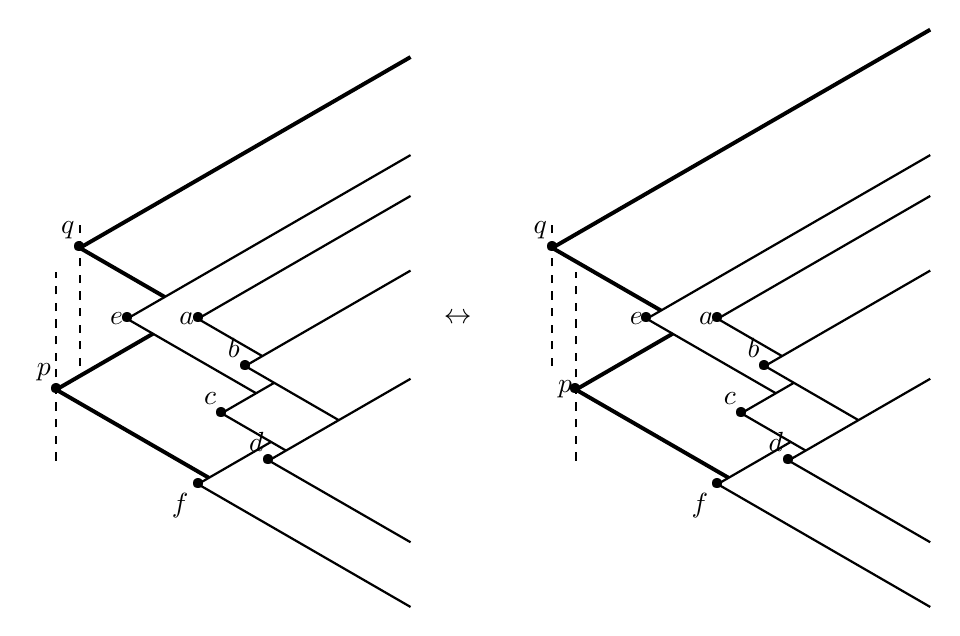
\begin{tikzpicture}[thick, scale=0.3]
        \node[label={[label distance = -3mm]160:$p$}] at
        (-1, 2.00) {\textbullet};
        \node[label={[label distance = -3mm]180:$e$}] at
        (2.00, 5.00) {\textbullet};
        \node[label={[label distance = -3mm]180:$a$}] at
        (5.00, 5.00) {\textbullet};
        \node[label={[label distance = -3mm]160:$b$}] at
        (7.00, 3.00) {\textbullet};
        \node[label={[label distance = -3mm]160:$c$}] at
        (6.00, 1.00) {\textbullet};
        \node[label={[label distance = -3mm]160:$d$}] at
        (8.00, -1.00) {\textbullet};
        \node[label={[label distance = -3mm]160:$q$}] at
        (0.00, 8.00) {\textbullet};
        \node[label={[label distance = -3mm]220:$f$}] at
        (5.00, -2.00) {\textbullet};

        % d cone
        \draw (8.00, -1.00) -- (14.00, -4.46);
        \draw (8.00, -1.00) -- (14.00, 2.46);
        % b cone
        \draw (7.00, 3.00) -- (10.96, 0.71);
        \draw (7.00, 3.00) -- (14.00, 7.04);
        % c cone
        \draw (6.00, 1.00) -- (8.73, -0.58);
        \draw (6.00, 1.00) -- (8.23, 2.29);
        % f cone
        \draw (5.00, -2.00) -- (14.00, -7.20);
        \draw (5.00, -2.00) -- (8.10, -0.21);
        % a cone
        \draw (5.00, 5.00) -- (7.73, 3.42);
        \draw (5.00, 5.00) -- (14.00, 10.20);
        % e cone
        \draw (2.00, 5.00) -- (7.46, 1.85);
        \draw (2.00, 5.00) -- (14.00, 11.93);
        % q cone
        \draw[line width = 0.5mm] (0.00, 8.00) -- (3.60, 5.92);
        \draw[line width = 0.5mm] (0.00, 8.00) -- (14.00, 16.08);
        % p cone
        \draw[line width = 0.5mm] (-1.00, 2.00) -- (5.46, -1.73);
        \draw[line width = 0.5mm] (-1.00, 2.00) -- (3.10, 4.37);

        \draw[dashed] (-1, -1) -- (-1, 7);
        \draw[dashed] (0, 3) -- (0, 9);

        \draw[dashed] (21, -1) -- (21, 7);
        \draw[dashed] (20, 3) -- (20, 9);

        \node at (16, 5) {$ \leftrightarrow$};

        \node[label={[label distance = -3mm]180:$p$}] at
        (21.00, 2.00) {\textbullet};
        \node[label={[label distance = -3mm]180:$e$}] at
        (24.00, 5.00) {\textbullet};
        \node[label={[label distance = -3mm]180:$a$}] at
        (27.00, 5.00) {\textbullet};
        \node[label={[label distance = -3mm]160:$b$}] at
        (29.00, 3.00) {\textbullet};
        \node[label={[label distance = -3mm]160:$c$}] at
        (28.00, 1.00) {\textbullet};
        \node[label={[label distance = -3mm]160:$d$}] at
        (30.00, -1.00) {\textbullet};
        \node[label={[label distance = -3mm]160:$q$}] at
        (20.00, 8.00) {\textbullet};
        \node[label={[label distance = -3mm]220:$f$}] at
        (27.00, -2.00) {\textbullet};

        % d cone
        \draw (30.00, -1.00) -- (36.00, -4.46);
        \draw (30.00, -1.00) -- (36.00, 2.46);
        % b cone
        \draw (29.00, 3.00) -- (32.96, 0.71);
        \draw (29.00, 3.00) -- (36.00, 7.04);
        % c cone
        \draw (28.00, 1.00) -- (30.73, -0.58);
        \draw (28.00, 1.00) -- (30.23, 2.29);
        % f cone
        \draw (27.00, -2.00) -- (36.00, -7.20);
        \draw (27.00, -2.00) -- (30.10, -0.21);
        % a cone
        \draw (27.00, 5.00) -- (29.73, 3.42);
        \draw (27.00, 5.00) -- (36.00, 10.20);
        % e cone
        \draw (24.00, 5.00) -- (29.46, 1.85);
        \draw (24.00, 5.00) -- (36.00, 11.93);
        % p cone
        \draw[line width = 0.5mm] (21.00, 2.00) -- (27.46, -1.73);
        \draw[line width = 0.5mm] (21.00, 2.00) -- (25.10, 4.37);
        % q cone
        \draw[line width = 0.5mm] (20.00, 8.00) -- (24.60, 5.35);
        \draw[line width = 0.5mm] (20.00, 8.00) -- (36.00, 17.24);
    \end{tikzpicture}
    \caption[Exemplo de evento \textsc{horizontal} em que nada acontece]{Se $p$ não está em $\Hits_{up}(q)$, ou se
    $q$ não está em $\Hits_{low}(p)$, nada acontece.}
    \label{fig:parcinetico:eventohorizontalabaixosemmudancas}
\end{figure}